% sh(x) = (e^x - e^(-x)) / 2
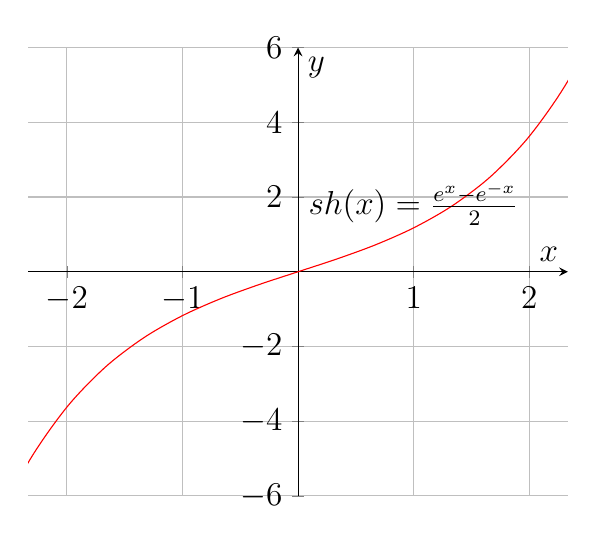
\begin{tikzpicture}
  \begin{axis}[domain=-4:4,ymin=-6,ymax=6, grid=both, font=\large, axis lines = middle, smooth, xlabel={$x$}, ylabel={$y$}]
    \addplot[draw=red] {(e^x - e^(-x)) / 2};
    \node at (axis cs:1,1.8) {$sh(x) = \frac{e^x - e^{-x}}{2}$};
  \end{axis}
\end{tikzpicture}
